\chapter{Time-dependent effects on the public goods game} %3P2
\label{chap:TimeEffects}



\begin{quotation}

	\vspace{-3cm}

    \begin{flushright}
    \begin{minipage}[t][5cm][b]{0.5\textwidth}
    {\letquote ``Time is the longest distance between two places."}
    
    \bigskip
    
    -{\small  Tennessee Williams}
    \end{minipage}
    \end{flushright}
    
    \vspace{0.5cm}
\end{quotation}




Understanding how individuals cooperate and form groups is fundamental to many fields, from biology to economics \cite{CoopBio,CoopEconomy}. When we study these interactions, we find that adding more people to a group the problem does not scale linearly, on the contrary it creates entirely new patterns of behavior that we couldn't predict by looking at individuals alone. These emerging patterns make the study of populations a fascinating example of complex systems dynamics, where simple rules can lead to intricate and surprising outcomes.

Social physics research has developed various tools to understand these patterns \cite{SocialPhy}, but one framework stands out as particularly powerful: Evolutionary Game Theory (EGT). This approach combines the mathematical precision of game theory with the dynamic nature of evolution, helping us understand how behaviors spread and change in populations over time.

One of the most intriguing questions EGT helps us explore is how altruism emerges. Why would individuals choose to help others at a cost to themselves? This seemingly counterintuitive behavior has been studied through various games, including the well-known rock-paper-scissors \cite{RPSCooperation}, the prisoner's dilemma \cite{Prisionero}, and the public goods game \cite{PublicGoods}.

In the public goods game (PGG) a community where each person can either contribute to shared resources, cooperate, or benefit without contributing, defect. Cooperators ($C$) contribute a unit amount to each of their groups, while defectors ($D$) contribute nothing. The collective contributions are then multiplied by an enhancement factor $r$ and then the sum is shared equally among all group members, regardless of their contributions. The enhancement factor $r$ accounts for the profit of a certain investment, including the benefits of working as a group with greater productivity than if individuals were working alone.

This setup creates an interesting dilemma: while everyone benefits when many people cooperate, individuals can gain more by defecting and letting others do the work. Cooperation only flourishes when the enhancement factor $r$ approaches the group size \cite{r/G}. Otherwise, defectors eventually dominate the population, leading to the "tragedy of the commons", a situation where pursuing individual interests leads to collective failure.


To encourage cooperation, societies often employ various mechanisms. These include allowing people to move between groups \cite{Migration}, maintaining reputations \cite{Reputation}, rewarding cooperators \cite{Reward}, or punishing those who don't contribute. Punishment can take different forms, from social exclusion \cite{SocialExclusion} to monetary fines \cite{Punish2}. Our work focuses on monetary punishment by introducing a third type of individual: punishers ($P$). These individuals not only contribute to the public good but also pay extra to penalize defectors. While punishers earn less than normal cooperators, since they bear the cost of punishment, their presence can make defection less attractive and thereby increase overall cooperation. However, maintaining cooperation requires a critical mass of punishers, as shown in \cite{SocialExclusion}.


Previous studies have assumed that the rules of the game remain constant over time. However, real-world situations rarely work this way. While some researchers have explored how allowing people to choose their group members affects outcomes \cite{EdgeRule}, few have investigated what happens when the fundamental parameters of the system change over time. The enhancement factor $r$ is particularly likely to fluctuate in real situations as of changes in the productivity of the investments. To understand these effects, we study what happens when $r$ oscillates sinusoidally over time. We chose this dependence as a simple pattern that can help us understand more complex variations.

Moreover, real-world actions rarely have immediate consequences, yet most studies assume instant punishment. We explore this by introducing a time delay $\tau$ as the intercept between the instant when someone defects and when they receive punishment. The effect on delay was previously studied with human subjects \cite{Late}, but with a sample much smaller than in our simulations.

Our research reveals two key findings. First, large amplitudes of oscillation in the enhancement factor make it harder for cooperation to persist. Second, delays in punishment also hinder cooperation. We also noticed that rapid fluctuations, similar to random noise, don't significantly affect outcomes.



\section{Model of the simulation}
\label{3model}




We implemented the public goods game as a spatial model where individuals interact with their neighbors in a square grid. Each individual participates in five different groups, with each group containing exactly five members ($G=5$). When an individual participates in a game, they receive a payoff, $\Pi^g$, based on their strategy and the strategies of others in that particular group. Their accumulated payoff, $\Pi$ comes from adding up their earnings from all five games they participated in, $\Pi=\sum_g^G \Pi^g$. This payoff is a measure of the fitness of an individual in the system.

Our simulation grid has $L$ cells on each side. We typically use $L=300$ unless specified otherwise. This means we're modeling a total population of $N=L^2$ individuals, distributed among cooperators ($N_C$), defectors ($N_D$), and punishers ($N_P$), so that $N=N_C+N_D+N_P$.

In nature and society, successful behaviors tend to spread, people often imitate strategies that seem to be working well for others. We model this through an imitation rule implemented in a Monte Carlo simulation. In each step, we randomly select an individual, $x$, and one of their neighbors $y$. After they've both played their games and received their payoffs, $x$ might adopt $y$'s strategy according to a probability that depends on the payoff of both. The probability follows the Fermi distribution:
\begin{equation}
W(s_x \rightarrow s_y)=\frac{1}{1+\exp[(\Pi_{x}-\Pi_{y})/K]},
\end{equation}
If $y$ is doing much better than $x$ ($\Pi_y >> \Pi_x$), the probability of $x$ adopting $y$'s strategy becomes very high. On the other hand, if $x$ is doing much better than $y$ ($\Pi_x$ >> $\Pi_y$), $x$ will likely keep their current strategy. When both are doing similarly well, the change becomes more random.

$K$ serves as a way to regulate this randomness that appears when adopting a strategy. Humans commit errors and are not purely driven by rationality. Therefore they do not always act to the best response. As $K \to 0$ the individuals always change the strategy if their payoff is smaller than the neighbor's. As $K \to \infty$ the probability of change is $1/2$, regardless of the payoff. As \cite{ValorK} suggests, we set $K=0.5$ as a fully representative value.

We define one Monte Carlo Step (MCS) as $N$ iterations, meaning that on average, each individual has had one opportunity to update their strategy. This represents one generation in our evolutionary timeline. 

The starting configuration of individual's strategies can change the outcome of the simulation. All the results presented in this paper come from randomly assigning strategies to individuals across the grid at the beginning. 




\section{The punishment methods: pool and peer punishment}
\label{3punish}



\begin{figure}
	\centering
	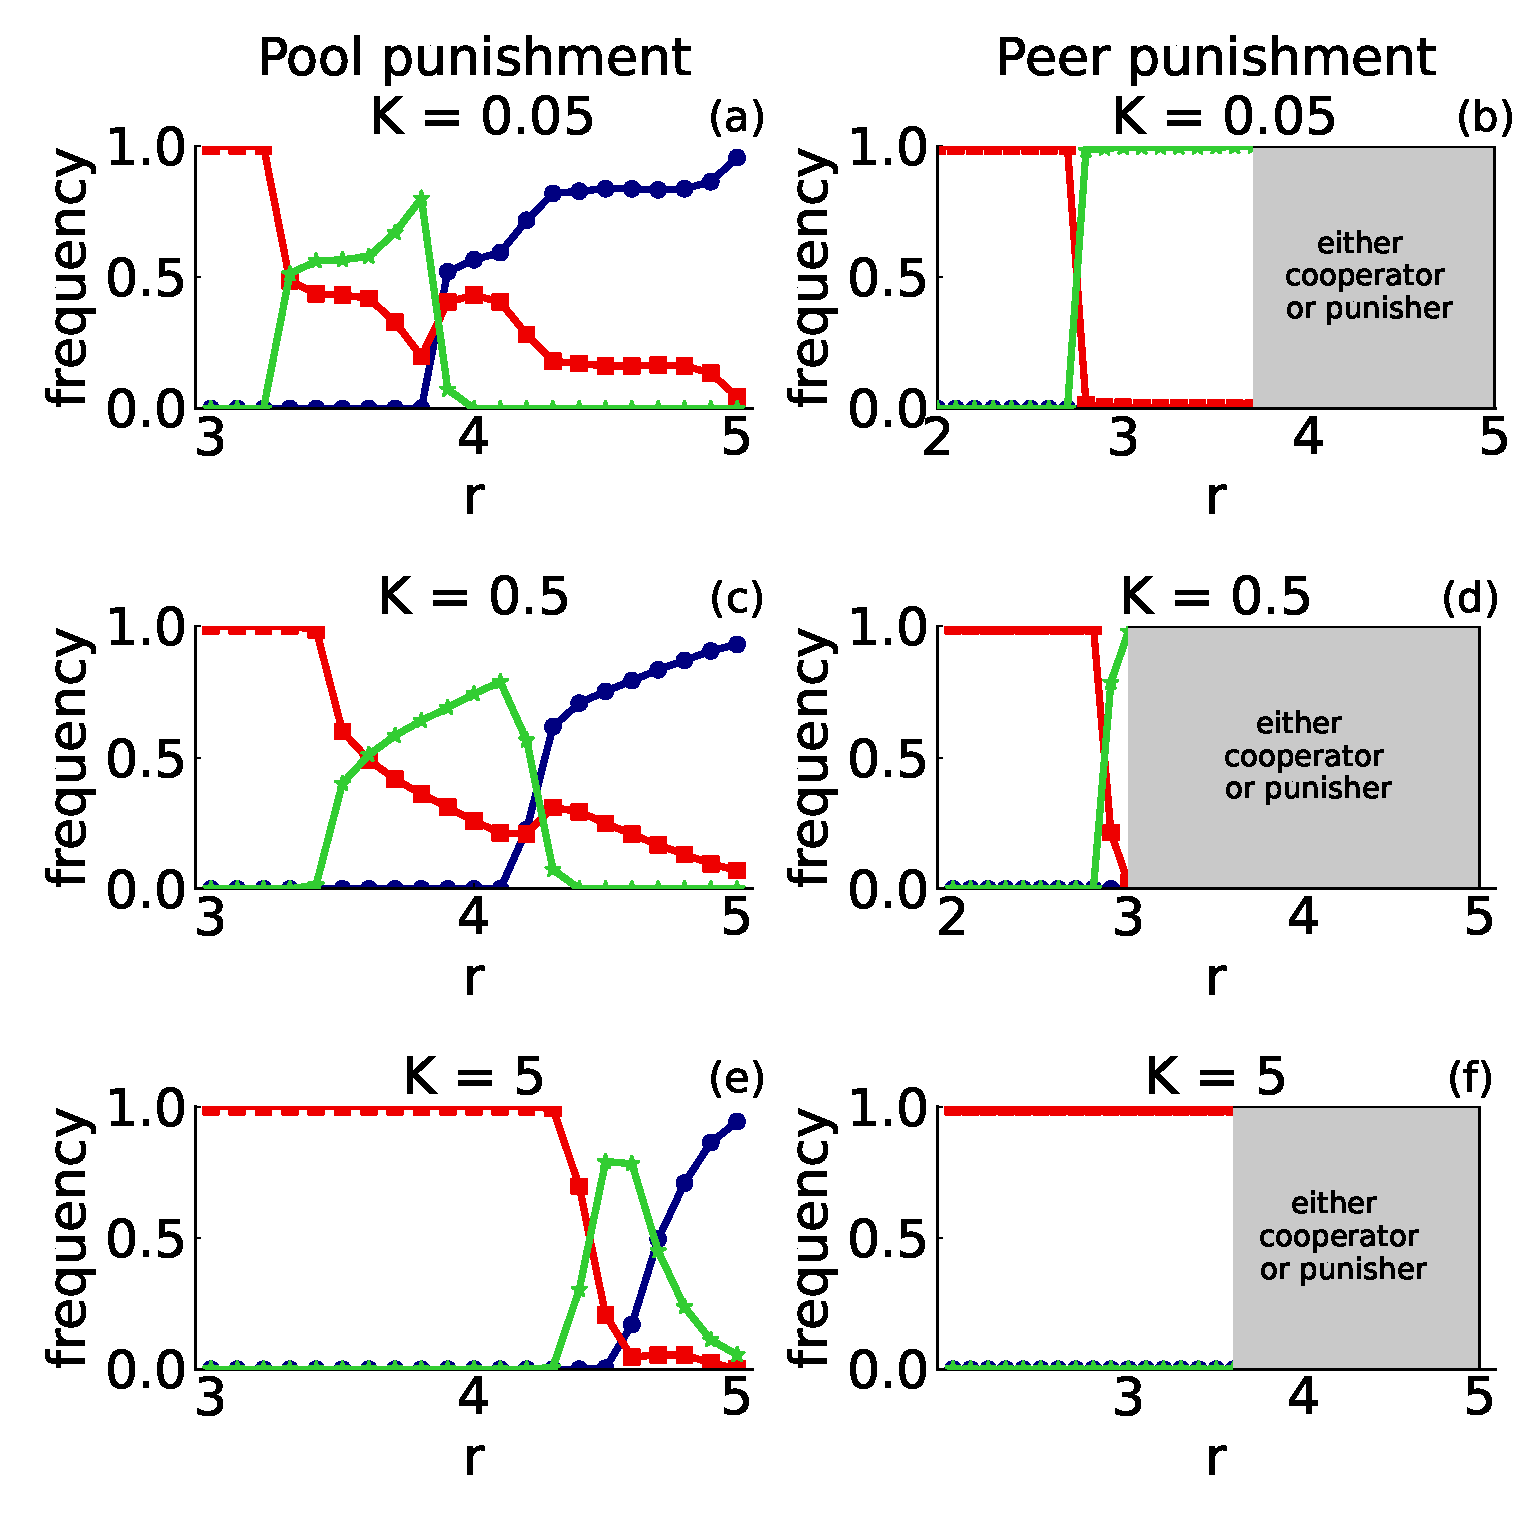
\includegraphics[width=1\linewidth]{Images/P2/densidadVSr_L300t5000variosK.eps}
	\caption{Frequency of each strategy after $5000$ MCS of a PGG simulation as a function of $r$ for different values of the stochastic noise regulator $K$. Cooperators in blue, defectors in red and punishers in green. For greater noise values, cooperation is less profitable. (b) (d) (f) For peer punishment, at some $r$ values defectors become extinct, so  punishers have the same payoff as cooperators. With sufficiently large relaxation times, either punishers or cooperators will go extinct as of neutral drift. (f) For $K=5$ the phase shift between whole domination from defectors and its extinction is very sudden (the step between consecutive $r$ values is $0.1$). The lines are used to guide the eye, and its width is larger than the corresponding error. We have used the following parameter values: $\beta=0.125$, $\gamma=0.0125$}
	\label{densidad}
\end{figure}




Societies have long used monetary fines to discourage undesirable behavior and promote cooperation. Think of parking tickets, environmental penalties, or business regulations. All these represent ways that communities punish those who don't cooperate with social rules. In our model, we explore two distinct approaches to implementing such punishment: pool punishment and peer punishment. 
In pool punishment, punishers contribute to a common fund. Each time punishers participate in the public goods game, they pay a small amount ($\gamma=0.0125$) into this communal punishment fund. When they encounters a defector, the defector must leave a fine ($\beta=0.125$). Importantly, this fine is applied only once per defector, regardless of how many punishers are in the group.

Peer punishment works differently. Instead of contributing to a central fund, punishers directly confront defectors. Each punisher pays a personal cost ($\gamma=0.0125$) to punish each defector they encounter, and each defector receives a separate fine ($\beta=0.125$) from each punisher. This can result in more severe punishment when multiple punishers are present.

Both approaches reflects different real-world systems for enforcing cooperation. Pool punishment reflects individuals reporting defectors to a gubernamental enforcement institution, paying taxes to maintaining it. Alternatively in peer punishment, the punishers take a more personal approach conflicting directly with the defectors.


These approaches lead to different mathematical expressions for how individuals fare in the game.

For pool punishment:
\begin{equation}\small
\begin{split}
\text{Cooperators earn: } &\Pi_C^g=\frac{r}{G}(N_C^g+N_P^g)-1 \\
\text{Punishers earn: } &\Pi_P^g=\frac{r}{G}(N_C^g+N_P^g)-1-\gamma \\
\text{Cooperators earn: } &\Pi_D^g = \left\{ \begin{array}{ll}
\frac{r}{G}(N_C^g+N_P^g) & \mbox{if $N_P^g=0$} \\
\frac{r}{G}(N_C^g+N_P^g)-\beta & \mbox{if $N_P^g\neq0$}.
\end{array}
\right\}
\end{split}
\end{equation}


For peer punishment, the equations change to reflect the multiple punishments possible:
\begin{equation}
\begin{split}
\text{Cooperators still earn: } &\Pi_C^g=\frac{r}{G}(N_C^g+N_P^g)-1 \\
\text{Punishers now earn: } &\Pi_P^g=\frac{r}{G}(N_C^g+N_P^g)-1-\gamma N_D^g \\
\text{Defectors earn: } &\Pi_D^g=\frac{r}{G}(N_C^g+N_P^g)-\beta N_P^g.
\end{split}    
\end{equation}



When we simulate these systems over $5000$ generations (Monte Carlo Steps), we observe how different strategies succeed under varying conditions in Figure \ref{densidad}. At low enhancement factors $r$, defection dominates because the benefits of cooperation aren't high enough to offset its costs. As $r$ increases, punishers begin to thrive because the greater benefits of cooperation make their enforcement role more valuable. At even higher r values, normal cooperators can sometimes outcompete punishers because the high returns make punishment less necessary.

The stochastic noise parameter K influences these patterns significantly. Higher noise levels make cooperation harder to maintain, shifting the transition points toward higher r values. This reflects how uncertainty or imperfect information can make maintaining cooperation more challenging.

Peer punishment shows some particularly interesting dynamics. Under certain conditions, defectors can be completely eliminated. When this happens, punishers and cooperators become equally successful since there's no one left to punish. Then, random chance eventually leads one strategy to dominate through what is called neutral drift. The outcome depends on the relative numbers of punishers and cooperators when defectors disappear, and possibly on their spatial distribution and the system's size.

Comparing the two punishment systems under the same fine $\beta$ and cost $\gamma$ values, peer punishment proves more effective at promoting cooperation. This makes intuitive sense since defectors face multiple fines under peer punishment, making the consequences of non-cooperation more severe.




\section{Varying the enhancement factor as oscillations on time}
\label{3oscillating}


\begin{figure}
	\centering
	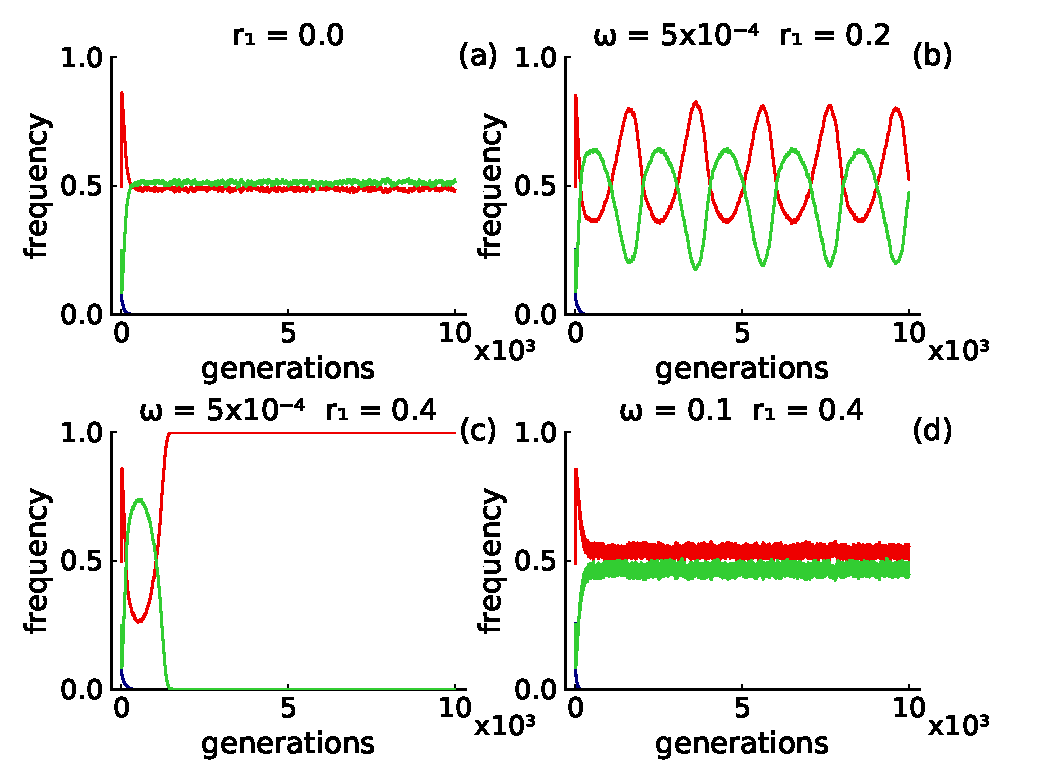
\includegraphics[width=1\linewidth]{Images/P2/freq_tiempo_T0seleccion_Pool.eps}
	\caption{Frequency of each strategy as time passes with an oscillating enhancement factor of the form $r=r_0+r_1\sin(\frac{2\pi \omega}{L^2}t+\delta)$, where  $r_0=3.6$ is the mean value of $r$, $\omega$ is the oscillation frequency in units of MCS$^{-1}$ and $\delta=0$. Results are made in the pool punishment. Cooperators in blue, defectors in red and punishers in green. (a) At the value of $r=3.6$ the punishers and defectors are almost on equal terms rapidly oscillating due to noise. (b) For small oscillation frequencies, the defectors and punishers periodically dominate one another, being the punishers the ones with a greater mean frequency. (c) The amplitude of the oscillation is so big that defectors completely dominate after one cycle. (d) As the oscillation frequency increases, the dynamics is more similar as compared to the case without any $r$ oscillation; while very quick $r$ oscillations, possibly another type of noise, are insignificant to final frequency. We have used the parameter values $\beta=0.125$, $\gamma=0.0125$}
	\label{oscila}
\end{figure}



\begin{figure}
	\centering
	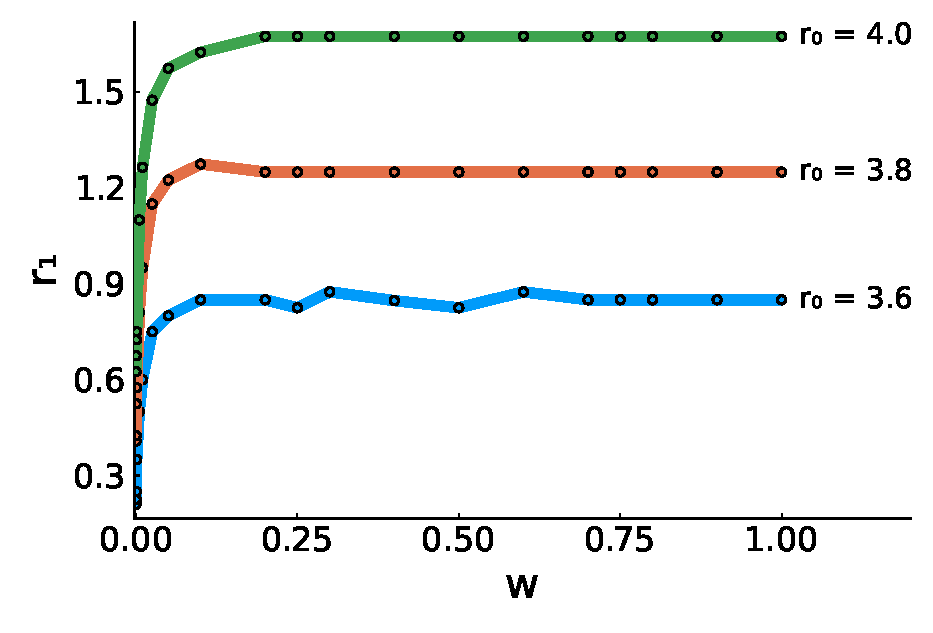
\includegraphics[width=1\linewidth]{Images/P2/grafica_r1_w0_T0_Pool.eps}
	\caption{The figure represents the amplitude $r_1$ of the oscillation $r=r_0+r_1\sin(\frac{2\pi\omega}{L^2}t+\delta)$ for different values of $r_0$, that limits the phase of only defectors (greater amplitudes) and defectors plus punishers (lower amplitudes) in the strict pool punishment regime with a punisher threshold $T=0$. The limiting amplitude $r_1$ grows as $r_0$ raises and, at low oscillation frequencies, when $\omega$ raises. The lines are used to guide the eye, and its width is comparable to the corresponding error. We have used the parameters: $\delta=0$, $\beta=0.125$, $\gamma=0.0125$}
	\label{r1_w0}
\end{figure}





In real societies, the benefits of cooperation rarely remain constant. Consider investing in a business venture: some days the market soars, other days it plunges. Another example of cooperative activity is farming, which experiences cycles of abundance and scarcity. The public goods game, as typically studied, simplifies this reality by assuming constant returns on cooperation. To better understand how these real-world fluctuations affect cooperation, we need to introduce time-varying returns into our model.

We model these changing investment returns by making the enhancement factor r oscillate over time. While real-world fluctuations can be complex, we start with a simple sinusoidal pattern that captures the essential behavior of periodic changes, a sinusoidal oscillation: $r=r_0+r_1\sin(\frac{2\pi\omega}{L^2}t)$

The frequency $\omega$, measured in inverse Monte Carlo Steps ($MCS^-1$), lets us explore different types of real-world fluctuations. Low frequencies might represent long-term economic cycles, while high frequencies could model rapid fluctuations like daily market volatility or random noise in the system.

When we examine how populations evolve under these oscillating conditions (shown in Figure \ref{oscila}), we discover that larger oscillations make it harder for cooperation to survive. When we increase the amplitude $r$, defectors gain an advantage, sometimes even taking over the entire population, as shown in Figure \ref{oscila}(c). This suggests that stability, in the sense of predictable returns on cooperation – plays a crucial role in maintaining cooperative behavior.

The frequency of oscillations also matters. When oscillations happen very quickly (Figure \ref{oscila}(d)), the population behaves almost as if there were no oscillations at all. This makes intuitive sense: if conditions change faster than people can adapt their strategies, they respond to the average conditions instead.

These findings hold true regardless of whether we use pool or peer punishment, and they persist across different levels of decision-making noise ($K$). The fundamental relationship between instability and reduced cooperation appears to be a robust feature of the system.

To understand exactly when defection becomes dominant, we created Figure \ref{r1_w0}. This figure shows the critical amplitude $r_1$ that separates regions where punishers can survive from regions where defectors completely take over, plotted against the oscillation frequency $\omega$ for different values $r_0$. The resulting curve reveals several key insights:

First, the critical amplitude increases with frequency until reaching a plateau. This means that faster oscillations need larger amplitudes to disrupt cooperation completely. At low frequencies, even small oscillations can lead to defector dominance because there are long periods when $r$ dips low enough for defectors to multiply significantly. As frequency increases, the system has less time to respond to each low-$r$ period, requiring larger amplitudes to achieve the same effect.

Second, higher baseline values of $r_0$ push the critical amplitude higher. This makes sense since when cooperation is more profitable on average, it takes larger disruptions to make defection the winning strategy.

We observed these patterns starting from $\omega = 0.00001$, our lowest tested frequency. Interestingly, at even lower frequencies, punishers dominate the system. This occurs because we start our simulations with $\delta = 0$, meaning $r$ initially increases, giving cooperation an early advantage that becomes decisive over very long oscillation periods.

This analysis reveals that cooperation is most vulnerable to slow, large-amplitude changes in the benefits of cooperation. Fast changes, even of large amplitude, have less impact because populations adapt to average conditions. These findings suggest that societies are more resilient to rapid fluctuations in cooperative benefits than to long-term cycles of boom and bust.



\section{Having a delay in punishment}
\label{3delay}



\begin{figure}
	\centering
	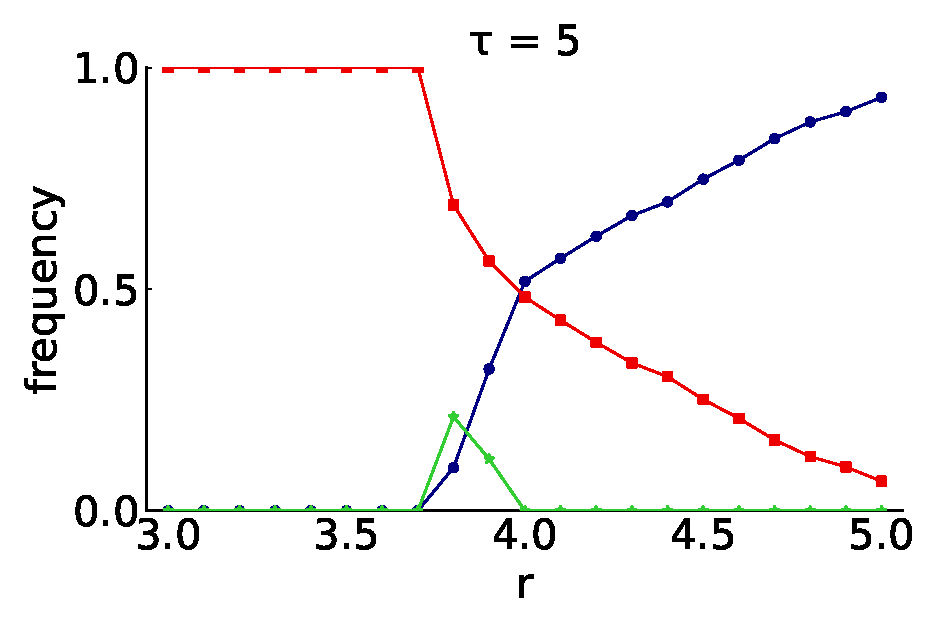
\includegraphics[width=1\linewidth]{Images/P2/densidad_retardo_tau5.0_L100_T0_t5000_Pool.eps}
	
	\caption{
	Frequency of each strategy averaged on the last iterations of a PGG simulation with a delay $\tau=5$ MCS when the defectors are charged with the fine as a function of $r$ in the pool punishment regime. Cooperators in blue, defectors in red and punishers in green. Punishers almost do not appear and defectors are more abundant than on Fig.~\ref{densidad}(c). The lines are used to guide the eye, and its width is larger than the corresponding error. We have used the parameters: $\beta=0.125$, $\gamma=0.0125$, $L=100$. }
	\label{freq_retardo}
\end{figure}

\begin{figure}
	\centering
	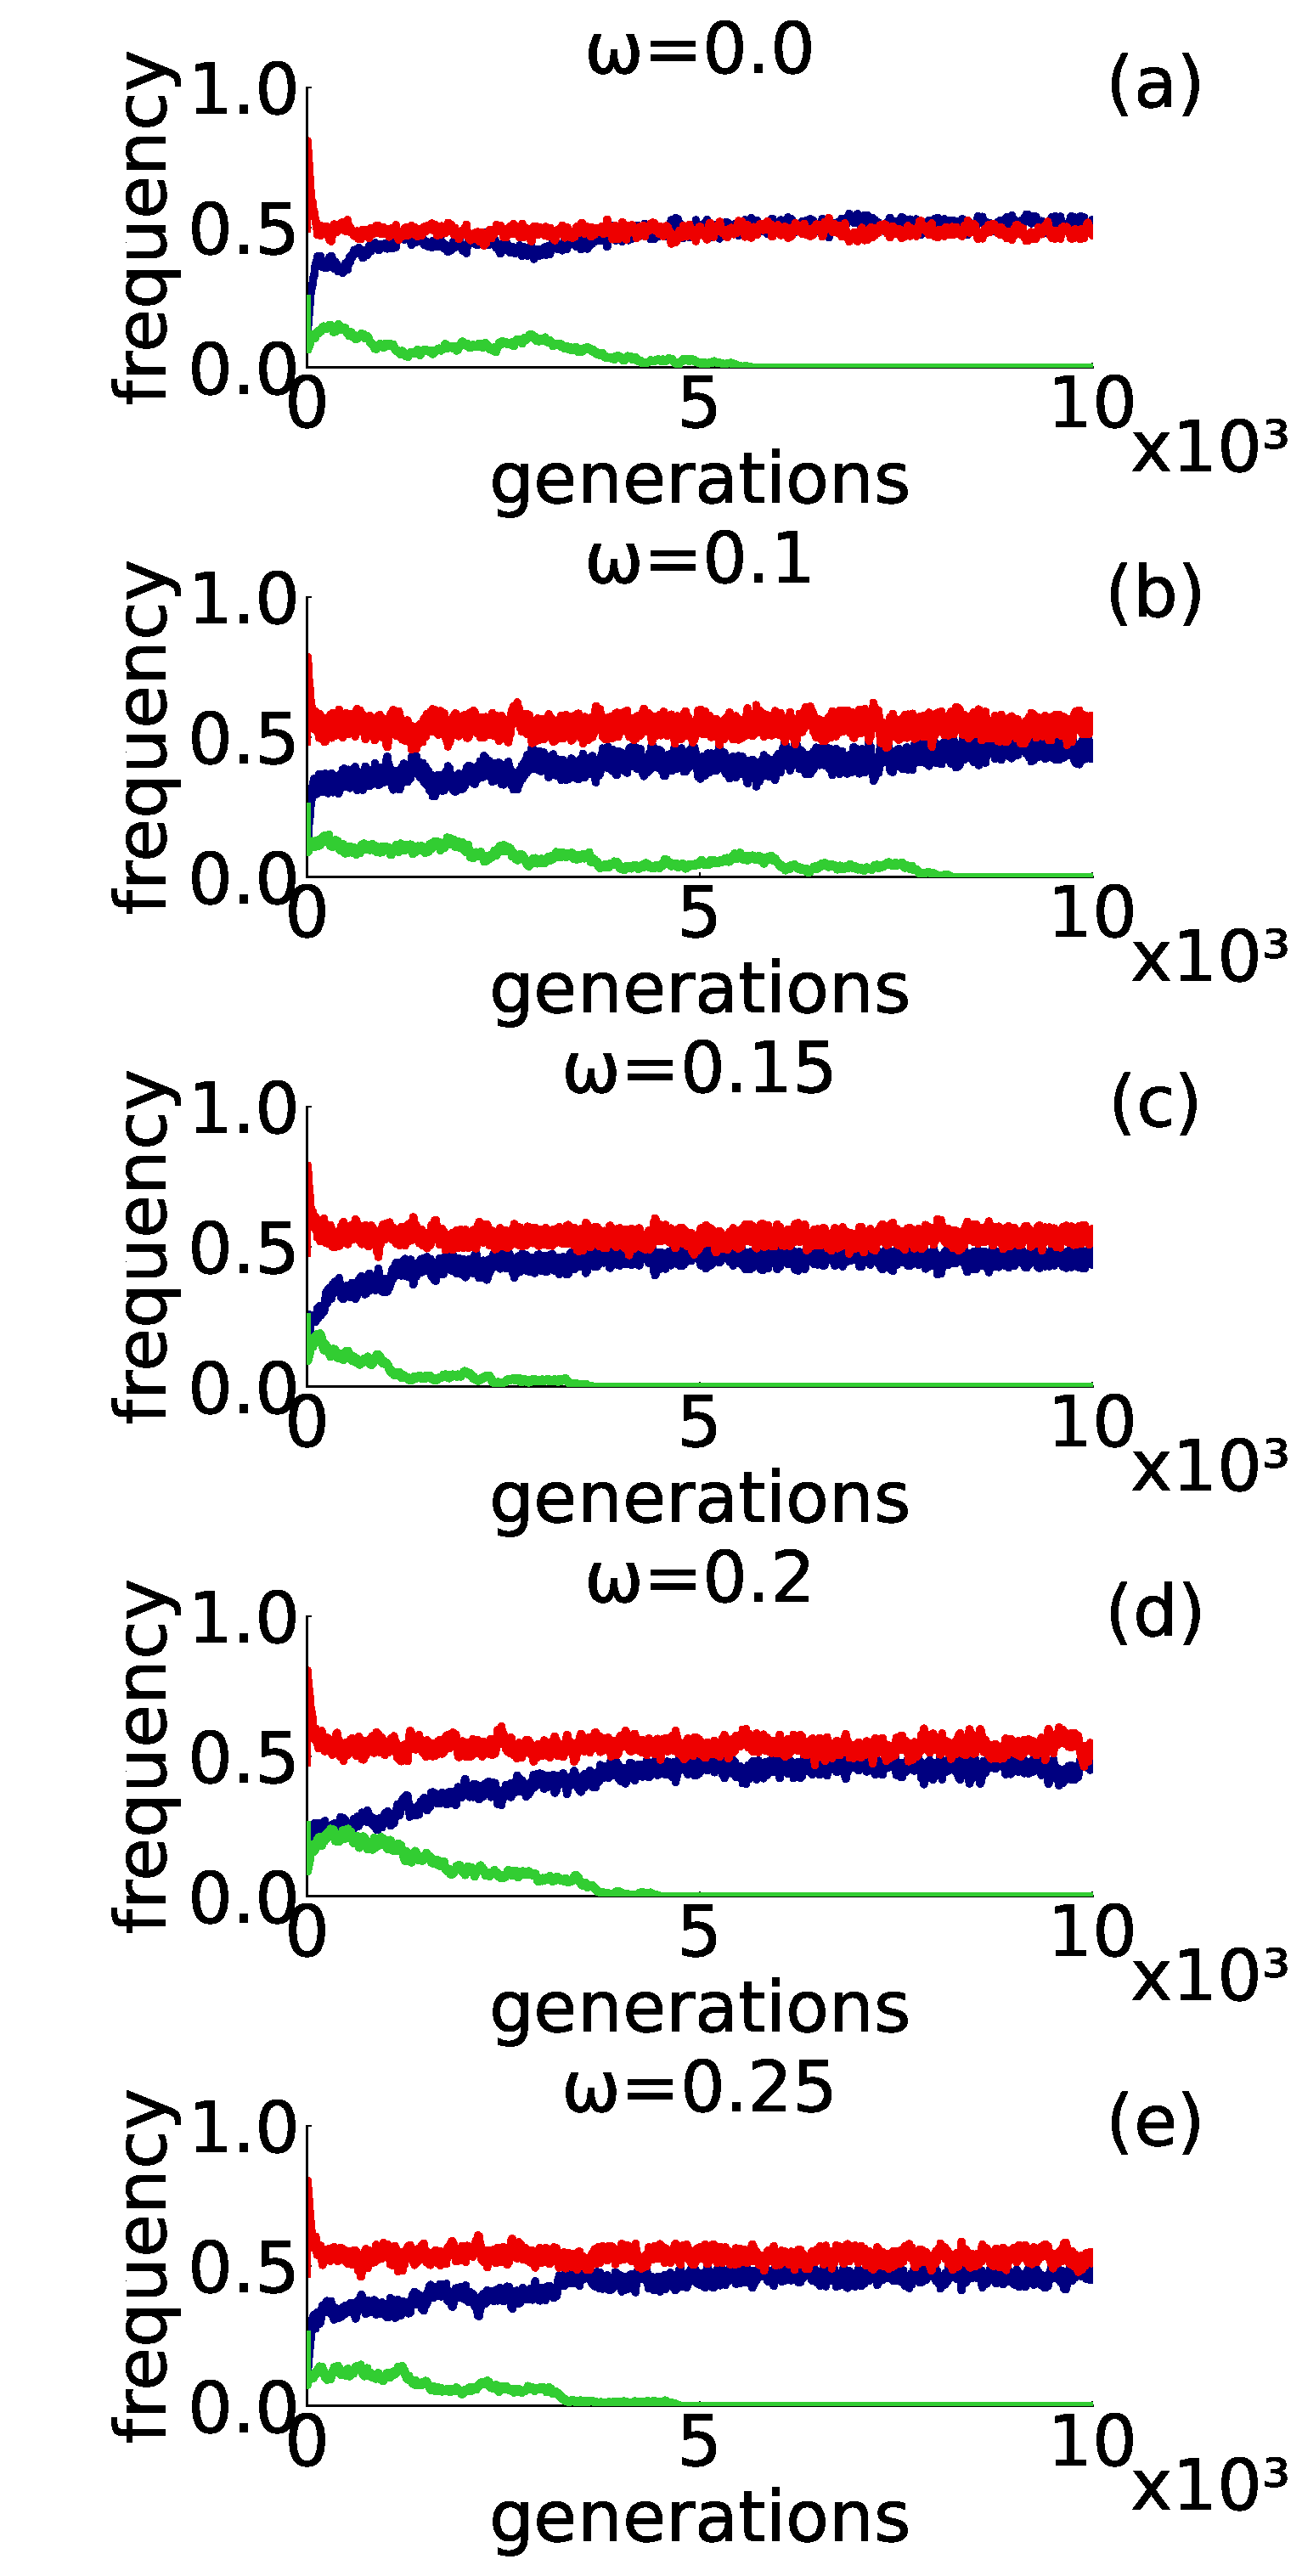
\includegraphics[width=0.6\linewidth]{Images/P2/freq_tiempo_retardoYsin_T0_r04.0_r10.5_tau50000_L100K0.5_t10000.eps}
	\caption{Frequency of each strategy as time passes of a PGG simulation with a delay $\tau=5$ MCS when the defectors are charged with the fine for different oscillation frequencies $\omega$ in the pool punishment regime. (a) No oscillation on the factor $r$. The oscillation of the frequency is due to the delay. With oscillation in the factor $r$, the (b-e) graphics look similar. There is no apparent difference in (d) although $w=0.2=1/\tau$ is the frequency we expected for a resonant behaviour. Cooperators in blue, defectors in red and punishers in green. We have used the parameters: $r_0=4.0$, $r_1=0.5$, $\beta=0.125$, $\gamma=0.0125$}
	\label{tiempo_retardo_oscilacion}
\end{figure}





In real life, actions and their consequences rarely happen simultaneously. When you speed on the highway, the ticket might arrive weeks later. This delay between action and consequence, or punishment, can significantly affect behavior. Understanding these effects is crucial for designing effective enforcement systems.

To explore how such delays influence cooperation, we modified our model to include a time lag so defectors stay some iterations of the game without receiving the punishment of their infringement.  Punishers detect defection and moments later, defectors actually pay their fines. This delay gives violators a temporary advantage as they can continue benefiting from their behavior before facing consequences.

The added complexity of tracking delayed punishments significantly increased computational demands, so we reduced our population size to L=100 to keep simulation times manageable. Even with this smaller population, the results proved illuminating.

Looking at Figure \ref{freq_retardo}, which shows the long-term frequency of each strategy with a delay of $\tau=5$ MCS, we see a dramatic shift from our previous results. Comparing this to Figure \ref{densidad}(c) (the no-delay case), we observe two significant changes: (1) Punishers have almost completely disappeared across most values of the enhancement factor $r$ (2) While normal cooperators appear at lower $r$ values than before, defectors maintain a much stronger presence

This weakening of cooperation makes intuitive sense when we consider how people learn and adapt their behavior. Just as children need to connect punishment directly with their actions to understand consequences, our simulated individuals become less likely to change their behavior when punishment is delayed. The longer the gap between action and consequence, the weaker the learning effect becomes. A principle that holds true whether we use peer punishment or vary the noise in decision-making.

To further understand these delay effects, we investigated whether they might interact with the oscillating returns we studied earlier. Figure \ref{tiempo_retardo_oscilacion} shows how populations evolve over time with both delay ($\tau=5$) and oscillating enhancement factors ($r_0=3.8$, $r_1=0.5$) at different frequencies. We were particularly interested in whether we might see resonance, a strengthening of effects, when the oscillation frequency matches the natural frequency created by the delay ($\omega=1/\tau=0.2$).

Nonetheless we found no evidence of such resonance. The population dynamics looked similar across different frequencies, even near the theoretical resonance point as seen in Fig.~\ref{tiempo_retardo_oscilacion}(d). Even more unexpectedly, we didn't observe the periodic oscillations we might have expected given our sinusoidal variation in returns.

What explains this lack of periodicity? Our first thought was that random noise in decision-making might be masking any periodic patterns. However, when we ran simulations in the noiseless regime ($K \to 0$), we still saw no periodic behavior. Then, another account for stocahasticity is the randomness of our Monte Carlo simulation. Specifically, in how we randomly choose which individuals get to update their strategies. This inherent randomness in the update process appears to overwhelm any periodic forcing from our oscillating enhancement factor. Another fact that restrains the observation of oscillation and resonance is the large value of $\omega$, as high-frequency oscillations do not provide with sufficient time for population to adapt. 

This finding highlights an important principle: while both delayed punishment and oscillating returns can independently weaken cooperation, their combined effects don't produce simple, predictable patterns, at least for the parameters studied. A further study with increased range of parameters for larger $\tau$ and smaller $\omega$ values is necessary.




\section{Conclusions }
\label{3Conclusions}


In this chapter, we examined time-dependent effects in the public goods game by adding an additional strategy, the punisher, among cooperators and defectors. Two forms of punishment, peer and pool punishment, were analyzed. While both punishment strategies yielded similar outcomes, peer punishment promoted cooperation more effectively. This greater efficacy comes from the fact that defectors are penalized multiple times for the same infraction, leading to a cumulative punishment effect.

To explore the dynamical nature of the game, we introduced a time-dependent enhancement factor $r$ and a time delay $\tau$ in the application of punishment to defectors. Both mechanisms were found to have a negative effect in cooperation. Large oscillation amplitudes led to an increase in the population of defectors, as oscillations in productivity disrupted the stability of cooperative behavior. For high oscillation frequencies, the system's behavior resembled that of a non-oscillatory scenario, suggesting that rapid oscillations, similar to noise, have minimal impact.

When a time delay in punishment was introduced, the effectiveness of punishment diminished, resulting in higher levels of defection. Thus, delayed punishment also impairs cooperation. 





\begin{thebibliography}{04}


\bibitem{SocialPhy} 
M. Jusup, P. Holme, K. Kanazawa, M. Takayasu, B. Podobnik, L. Wang, W. Luo, T. Klanjšček, J. Fan, S. Boccaletti, and M. Perc, Social Physics, Phys. Rep. \textbf{948}, 1 (2022). \url{https://doi.org/10.1016/j.physrep.2021.10.005}.

\bibitem{RPSCooperation} 
Z. Bi and H. Zhou, Optimal Cooperation-Trap Strategies for the Iterated Rock-Paper-Scissors Game, PLoS One \textbf{9}, e111278 (2014). \url{https://doi.org/10.1371/journal.pone.0111278}.

\bibitem{Prisionero} 
G. Szabó and C. Töke, Evolutionary Prisoner’s Dilemma Game on a Square Lattice, Phys. Rev. E \textbf{58}, 69 (1998). \url{https://doi.org/10.1103/PhysRevE.58.69}.

\bibitem{PublicGoods} 
M. Archetti and I. Scheuring, Game Theory of Public Goods in One-Shot Social Dilemmas Without Assortment, J. Theor. Biol. \textbf{299}, 9 (2012). \url{https://doi.org/10.1016/j.jtbi.2011.06.018}.

\bibitem{r/G} 
T. Wu, F. Fu, and L. Wang, Partner Selections in Public Goods Games with Constant Group Size, Phys. Rev. E \textbf{80}, 026121 (2009). \url{https://doi.org/10.1103/PhysRevE.80.026121}.

\bibitem{EdgeRule} 
X. Sun, Y. Li, H. Kang, Y. Shen, J. Peng, H. Wang, and Q. Chen, Co-Evolution of Complex Network Public Goods Game under the Edges Rules, MDPI Entropy \textbf{22}, 199 (2020). \url{https://doi.org/10.3390/e22020199}.

\bibitem{Migration} 
D. Helbing and W. Yu, The Outbreak of Cooperation among Success-Driven Individuals under Noisy Conditions, Proc. Natl. Acad. Sci. U.S.A. \textbf{106}, 3680 (2009). \url{https://doi.org/10.1073/pnas.0811503106}.

\bibitem{Reputation} 
Z. Wang, L. Wang, Z. Yin, and C. Xia, Inferring Reputation Promotes the Evolution of Cooperation in Spatial Social Dilemma Games, PLoS One \textbf{7}, e40218 (2012). \url{https://doi.org/10.1371/journal.pone.0040218}.

\bibitem{Reward} 
Y. Li, S. Chen, and B. Niu, Reward Depending on Public Funds Stimulates Cooperation in Spatial Prisoner’s Dilemma Games, Chaos Solitons Fractals \textbf{114}, 38 (2018). \url{https://doi.org/10.1016/j.chaos.2018.07.002}.

\bibitem{SocialExclusion} 
T. Sasaki and S. Uchida, The Evolution of Cooperation by Social Exclusion, Proc. R. Soc. B \textbf{280}, 20122498 (2013). \url{https://doi.org/10.1098/rspb.2012.2498}.

\bibitem{Punish2} 
A. Szolnoki, G. Szabó, and M. Perc, Phase Diagrams for the Spatial Public Goods Game with Pool Punishment, Phys. Rev. E \textbf{83}, 036101 (2011). \url{https://doi.org/10.1103/PhysRevE.83.036101}.

\bibitem{Late} 
I. Waichman and L. Stenzel, When Punishment Strikes Late: The Effect of a Delay in Punishment and Punishment Feedback on Cooperation and Efficiency, J. Neurosci. Psychol. Econ. \textbf{12}, 1 (2019). \url{https://doi.org/10.1037/npe0000099}.

\bibitem{ValorK} 
A. Szolnoki, M. Perc, and G. Szabó, Topology-Independent Impact of Noise on Cooperation in Spatial Public Goods Games, Phys. Rev. E \textbf{80}, 056109 (2009). \url{https://doi.org/10.1103/PhysRevE.80.056109}.



\end{thebibliography}






